\documentclass[11pt]{article}
% Single-column readable draft (NOT the ACL two-column layout). To produce the
% camera-ready, swap the geometry/natbib block below back for
% \usepackage[review]{acl} and restore the \And author form.
\usepackage[margin=1.1in]{geometry}
\usepackage{times}
\usepackage{latexsym}
\usepackage[T1]{fontenc}
\usepackage[utf8]{inputenc}
\usepackage{microtype}
\usepackage{graphicx}
\usepackage{xcolor}
\usepackage{booktabs}
\usepackage{amsmath}
\usepackage{natbib}
\usepackage[hidelinks]{hyperref}
\setlength{\parskip}{0.4em}

% Resolve figures relative to this file (reports/) so includes find the repo dirs.
\graphicspath{{../}{../experiments/}{../img/}}

\newcommand{\am}[1]{\textcolor{orange}{[AM: #1]}}
\newcommand{\jb}[1]{\textcolor{blue}{[JB: #1]}} % draft notes / open items

\title{Read, Translate, Write: LLMs Translate with Fuzzy Semantic Hubs}
\author{First Author \and Second Author}

% =====================================================================
% DRAFT v5 (auto-assembled). Fleshes out the two empirical sections the
% intro promises: (1) the linear model from monolingual competence to
% translation (H1), and (2) GCM head/feature identification + the
% Multi-BLiMP head-ablation follow-up (H4). Intro/Related/§5(finetuning,
% H3, external) are kept as stubs -- copy the finished prose from v4.tex.
% Numbers are sourced from experiments/*/REPORT.md and the run outputs;
% see reports/P1_overview.md for the full provenance and validity flags,
% and PAPER_TODO.md for figures/items still pending.
% =====================================================================

\begin{document}
\maketitle
\begin{abstract}
\jb{Abstract last. One line: translation quality has strong separable
source/target structure, though the measured FLORES-perplexity linear fit is
weak (H1 caveat); the components that distinguish good from bad translations
overlap with sparse features the model uses to represent grammar monolingually
(H4); and collaborator-owned finetuning results should state H3 once verified.
Convergent, not conclusive, evidence that LLMs translate by reusing
language-modeling machinery through a multilingual ``semantic hub.''}
\end{abstract}

\section{Introduction}
\jb{Use the v4.tex introduction verbatim; it already states the stages-of-inference
framing and the three implications H1--H3 (and H4). Not reproduced here.}

\section{Related Work}
\jb{From v4.tex.}

% =====================================================================
\section{Monolingual Competence Predicts Translation Performance}
\label{sec:linear}

How much of a model's ability to translate is explained by its monolingual
language-modeling competence in the source and target languages, taken in
isolation? If translation reuses general language-modeling machinery, then a
model's BLEU on a language pair $(S,T)$ should be largely a function of two
monolingual quantities---competence in $S$ and competence in $T$---with no
language-pair-specific interaction term required (H1).

\paragraph{Setup.} We proxy monolingual competence with corpus perplexity on the
FLORES devtest split \citep{goyal2022flores}. The repo also computes
Multi-BLiMP accuracy/PER \citep{jumelet2025multiblimp}, but the OLS coefficients
reported below use the FLORES-perplexity columns in
\texttt{combined\_results\_\{model\}.csv}. For each ordered pair $(S,T)$ we take
$l_S, l_T$ and fit an ordinary least squares model
\begin{equation}
\hat{t}_{ST} = a + \beta_S\, l_S + \beta_T\, l_T,
\label{eq:linear}
\end{equation}
and, for contrast, a bilinear variant adding an interaction term
$\beta_{ST}\, l_S l_T$. Under H1 the interaction should add little: the bilinear
model should not substantially out-predict Eq.~\ref{eq:linear}. We report
results for Llama-3.1-8B and Aya-23-8B.

\paragraph{A linear-in-perplexity fit is weak\dots} The coefficients carry the right
sign---higher perplexity predicts lower BLEU ($\beta_S,\beta_T < 0$)---but the
linear model explains little variance: $R^2 = 0.02$ (Llama), $0.10$ (Aya), with
a mean absolute error of roughly $5$--$6$ BLEU points and predictions clustered
near the intercept. Taken alone, a linear-in-perplexity model is a poor BLEU
predictor.

\paragraph{\dots but the BLEU surface is rank-1.} A measured perplexity proxy is
not the only way to operationalize H1. We assemble the $(S,T)$ BLEU matrix $M$
and ask how well a single rank-1 factor reconstructs it,
$\text{faithfulness} = 1 - \lVert M - M_1\rVert_F / \lVert M\rVert_F$,
where $M_1$ is the leading SVD component. A rank-1 matrix is exactly separable
into source and target factors, $M_1(S,T)=f(S)g(T)$; this is a no-pair-specific
residual test, not the same additive no-interaction model as
Eq.~\ref{eq:linear}. We find rank-1 faithfulness of $\mathbf{88.3\%}$ (Llama)
and $82.4\%$ (Aya) on a $24\times24$ BLEU matrix with $24$ missing/self cells
imputed by column mean. The translation surface is therefore strongly
separable, even if our measured perplexity features do not recover the factors
well.

These metrics are not directly comparable, but they point in different
practical directions: measured FLORES perplexity has little linear predictive
power, while the BLEU matrix itself has a strong low-rank source/target
structure. We read this as evidence that FLORES perplexity is a \emph{noisy
proxy} for the competence factors the rank-1 decomposition recovers directly
from BLEU, rather than as evidence against H1.
\jb{This reconciliation is currently an assertion; tying the rank-1 left/right
factors back to a measured competence quantity would make it a result. See
PAPER\_TODO A1.}

\begin{figure}[t]
\centering
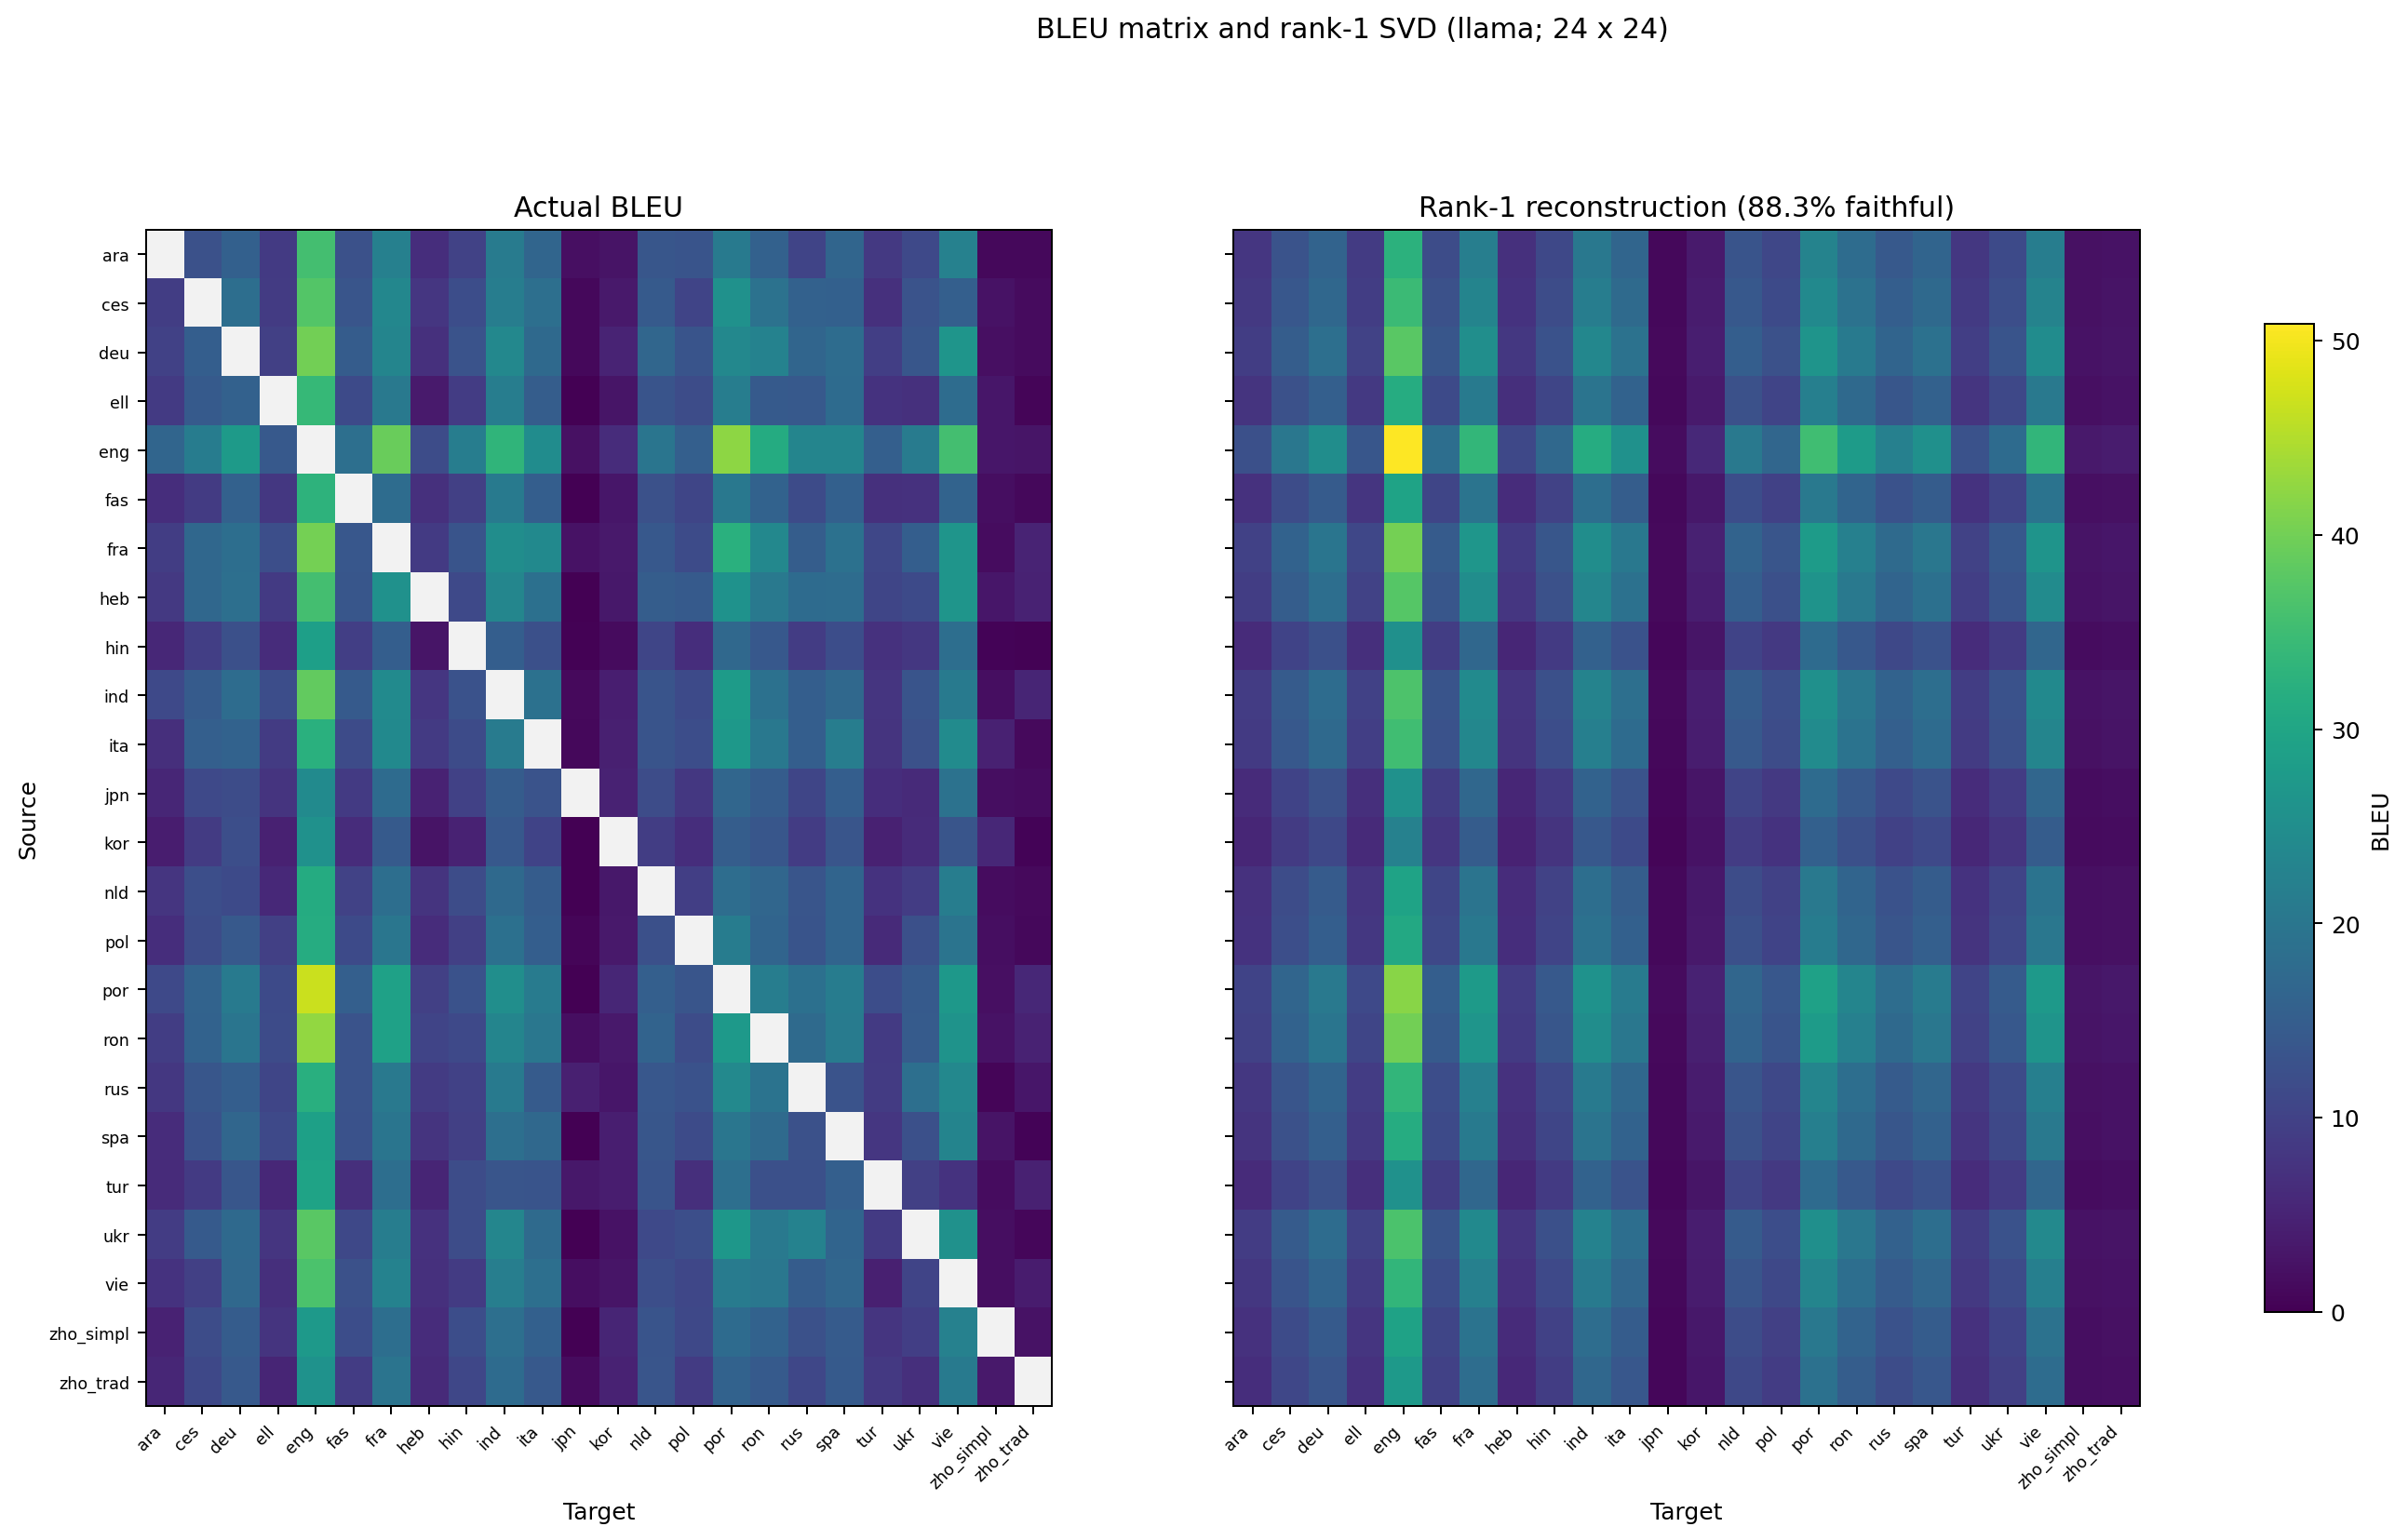
\includegraphics[width=\linewidth]{img/perplexity_bleu_linear/bleu_matrix_rank1_llama.png}
\caption{Raw Llama BLEU matrix and its rank-1 SVD reconstruction, computed from
the same \texttt{combined\_results\_llama.csv} pivot used for the $88.3\%$
faithfulness claim. The matrix is $24\times24$; $24$ missing cells are imputed
with target-column means for the SVD. Produced by
\texttt{rank1\_approximation.py}.
\jb{The mean-imputation can inflate the low-rank fit; recompute faithfulness on
observed cells only / diagonal excluded (PAPER\_TODO A1).}}
\label{fig:rank1}
\end{figure}

\begin{figure}[t]
\centering
\includegraphics[width=\linewidth]{img/perplexity_bleu_linear/llama_joint_competence_scatter.png}
\caption{Joint source$\times$target competence vs.\ BLEU (Llama); each point is a
language pair. Produced by \texttt{visualize\_correlation.py} from
\texttt{combined\_results\_llama.csv}.
\jb{Marked for P2 finalization in your A1 notes; included here so the section's
figure set is complete.}}
\label{fig:joint-competence}
\end{figure}

% =====================================================================
\section{Translation-Relevant Components Overlap With Language-Modeling Machinery}
\label{sec:gcm}

We now ask, mechanistically, \emph{which} model components carry the information
that distinguishes a correct translation from an incorrect one, and whether
those components are translation-specific or shared with monolingual language
modeling (H4). We proceed in two steps: (i) identify the influential components
with Generative Causal Mediation (GCM) on translation pairs
(\S\ref{sec:gcm-id}), then (ii) test whether the heads GCM implicates also carry
\emph{monolingual} grammatical information, by ablating them on Multi-BLiMP
minimal pairs (\S\ref{sec:gcm-ablate}).

\subsection{Identifying influential components with GCM}
\label{sec:gcm-id}

\paragraph{Background: indirect effects.} We want a \emph{causal} measure of how
much one internal component matters for the model's choice between two
translations. Fix a contrastive triple $(p_{\text{orig}}, r_{\text{orig}},
r_{\text{cf}})$---one prompt and two candidate continuations---and define the
preference metric
\begin{equation}
M = \log \pi(r_{\text{cf}}\mid p_{\text{orig}}) - \log \pi(r_{\text{orig}}\mid p_{\text{orig}}),
\label{eq:metric}
\end{equation}
where $\log\pi(r\mid p) = \sum_t \log p(r_t \mid p, r_{<t})$ is the
teacher-forced log-probability of a continuation, summed over its tokens (in
nats). $M$ is thus the model's log-odds preference for $r_{\text{cf}}$ over
$r_{\text{orig}}$ under the \emph{same} prompt. Now single out one component---an
attention head's output contribution, or one SAE feature---with activation $z$,
and write $M(z)$ for the metric as a function of that one activation while the
rest of the forward pass is held at its original-run values. The component takes
the value $z_{\text{orig}}$ on the original run and $z_{\text{cf}}$ on a run
where the model instead reads the counterfactual source. In the language of
causal mediation, the component is a \emph{mediator}, and its \emph{indirect
effect} is the change in $M$ caused by moving it between these two values---which
is exactly what activation patching measures, at a cost of one forward pass per
component:
\begin{equation}
\mathrm{IE}_{\text{patch}}(z) = M(z_{\text{orig}}) - M(z_{\text{cf}}).
\label{eq:patch}
\end{equation}

\paragraph{The GCM estimator.} GCM \citep{sankaranarayanan2026gcm} removes the
per-component cost by linearizing $M$ around $z_{\text{orig}}$. A first-order
Taylor expansion gives $M(z_{\text{cf}}) \approx M(z_{\text{orig}}) + \nabla_z
M|_{z_{\text{orig}}}\!\cdot(z_{\text{cf}} - z_{\text{orig}})$; substituting into
Eq.~\ref{eq:patch},
\begin{equation}
\widehat{\mathrm{IE}}(z) = \nabla_z M\big|_{z=z_{\text{orig}}} \cdot (z_{\text{orig}} - z_{\text{cf}}).
\label{eq:ie}
\end{equation}
This recovers $\mathrm{IE}_{\text{patch}}$ to first order but is computable for
\emph{every} component at once: the gradients $\nabla_z M$ come from a single
backward pass, and the deltas $(z_{\text{orig}} - z_{\text{cf}})$ from caching
each component's activation on the original and counterfactual runs. So one
forward$+$backward pass yields an IE estimate for all $1024$ heads and all
$32{,}768$ SAE features, versus one patched forward pass \emph{each} for the
exact version.

\paragraph{Reading magnitude and sign.} $\widehat{\mathrm{IE}}$ is in nats. Its
magnitude $|\widehat{\mathrm{IE}}|$ is how much the component, on its own, shifts
the preference between the two continuations; we rank components by
$\mathrm{mean}\,|\widehat{\mathrm{IE}}|$ over the $100$ pairs. Its sign---under
this orig-minus-cf convention, with $M = m_{\text{cf}} - m_{\text{orig}}$---says
which continuation the component favors in its original state: a positive
$\widehat{\mathrm{IE}}$ means the original activation (relative to the
counterfactual) pushes the model toward $r_{\text{cf}}$; a negative value means
it pushes toward the gold response $r_{\text{orig}}$. Section~\ref{sec:gcm-ablate}
turns on exactly this sign.\footnote{A first-order estimate is only as good as
the linearization. The repo's finite-difference test checks
$M(z_{\text{orig}}+\varepsilon\,\delta) - M(z_{\text{orig}}) \approx
\varepsilon\,\nabla_z M\cdot\delta$ per pair; it is currently \texttt{xfail}
(see PAPER\_TODO A2), so the linearization is taken on faith pending that check.}

\paragraph{Contrastive pairs from translation.} Rather than hand-written
contrasts, we use FLORES sentence pairs: $r_{\text{orig}}$ is the gold
translation of the original source, $r_{\text{cf}}$ the gold translation of a
different (counterfactual) source, both scored under the same prompt
$p_{\text{orig}}$. We attribute every attention head ($32\times32$ query-head
outputs, sliced from \texttt{o\_proj.input}) and every layer-16 SAE feature
($32{,}768$ features of \texttt{jbrinkma/sae-llama-3-8b-layer16}), patching at
the \emph{last source-token position} only. We sweep all $56$ ordered
cross-language directions among
\{eng, spa, deu, fra, tur, ara, hin, heb\}, nominally $100$ pairs per direction
(eng$\to$fra has $98$ successful pairs), on a 2-shot prompt.\footnote{Two
implementation points the method depends on: each
pair is scored in \emph{two} separate single-invoke traces (not one batched
multi-invoke trace, which left-pads and would shift the patched index); and
because writing to a module \emph{input} is unsupported, the per-head patch is
applied as the equivalent additive delta $(z-z_{\text{orig}})W_o^{\!\top}$ at
\texttt{o\_proj.output}.}

\paragraph{Control tasks.} The central methodological device is a $2\times2$
factorial that subtracts away two confounds---generic content discrimination
and cross-language routing---so the residual is attributable to a translation
circuit. The factors are \emph{cross} vs.\ \emph{same} (whether $S\!\neq\!T$, so
the model must route across languages) and \emph{real} vs.\ \emph{null} (whether
one scored response is the gold translation of the source, providing a
correctness anchor; in the \emph{null} condition both responses are gold
translations of \emph{other} sentences). The resulting subtractions are:
$\textsc{real\_cross}-\textsc{null\_cross}$ (translation-circuit-specific),
$\textsc{null\_cross}-\textsc{null\_same}$ (cross-language routing), and
$\textsc{real\_same}-\textsc{null\_same}$ (monolingual identity completion).
\textsc{null\_same}, where both responses are arbitrary same-language contents,
is the pure content-discrimination floor.

\paragraph{Sanity checks.} The identity patch ($z=z_{\text{orig}}$) reproduces
the unpatched metric to within bf16 round-off (drift $=0.0$ across all $56$
directions); the clean model prefers the gold over the counterfactual response
in $\geq99\%$ of pairs (length-normalized); and the top-$20$ head set is stable
under bootstrap resampling (inclusion frequency $0.92$--$1.00$). \jb{The
finite-difference linearization test is currently \texttt{xfail}, and the
ACP-vs-ATP interventional faithfulness check has not been run on the sweep; see
PAPER\_TODO A2.}

\paragraph{Result: heads look universal, but are mostly content.} Counting how
often each head lands in a direction's top-$20$, two heads (L17H21, L30H25)
appear in \emph{all $56$} directions, and the top-$20$ is dominated by late
layers (L28--L31); one SAE feature (f20383) is universal across all $56$
directions as well. Taken at face value this suggests shared ``universal
translation heads.'' The control tasks, however, substantially revise this
reading at the head level: the translation-circuit-specific contribution
$(\textsc{real\_cross}-\textsc{null\_cross})$ for the top heads is at most
$+0.025$ nat---at the bf16 noise floor. L30H25 is illustrative: its
$\textsc{real\_cross}$ effect ($+0.48$) is dwarfed by its $\textsc{null\_same}$
effect ($+1.21$), i.e.\ it fires \emph{more} in monolingual same-language
completion than in translation. At the head level it is a content head, not a
translation head.

\paragraph{Result: the sparse-feature signal is cleaner.} The same
decomposition at the SAE-feature level separates better. Feature f31444 is
nearly silent in monolingual completion ($\textsc{null\_same}\approx0.0002$) but
has substantial cross-language signal ($\textsc{real\_cross}=0.084$), roughly
half of it translation-specific---the cleanest translation-relevant component we
find. Moreover, of the $50$ most direction-universal SAE features, $9$ also
belong to an independently-defined set of grammatical-concept features
(\S\ref{sec:gcm-ablate} \jb{/ cross-ref the input-feature work}), versus
$\approx0.33$ expected by chance---a $\sim$27$\times$ enrichment. The features
the model relies on to translate are disproportionately the same features it
uses to represent grammar monolingually, consistent with a shared multilingual
``semantic hub'' (H4/H2).

\begin{figure}[t]
\centering

\includegraphics[width=\linewidth]{experiments/gcm_translation/img/three_way_decomposition_sae_full.png}
\caption{SAE-feature three-way decomposition. Per top feature, the mean
$|\widehat{\mathrm{IE}}|$ under \textsc{real\_cross}, \textsc{null\_cross}, and
\textsc{null\_same}, and the derived translation-circuit contribution. f31444 has
$\textsc{null\_same}\approx0$. Produced by \texttt{three\_way\_decomposition.py}
(full view: 56 cross-lang $+$ 8 same-lang directions).
\jb{Foreground the SAE figures over the head version (the head one is at the
noise floor); a head companion can go to the appendix. See PAPER\_TODO A2.}}
\label{fig:gcm-decomp}
\end{figure}

\begin{figure}[t]
\centering

\includegraphics[width=\linewidth]{experiments/gcm_translation/img/meeting_sae_grammar_overlap.png}
\caption{The $50$ most direction-universal layer-16 SAE features, by number of
the $56$ directions in which each appears in the top-$20$; red bars mark
features that also belong to the grammar-feature set ($9/50$ overlap vs.\
$\approx0.33$ by chance). Produced by \texttt{meeting\_plots.py} from the
cross-direction aggregation in \texttt{analyze.py}.}
\label{fig:gcm-grammar}
\end{figure}

\begin{figure}[t]
\centering
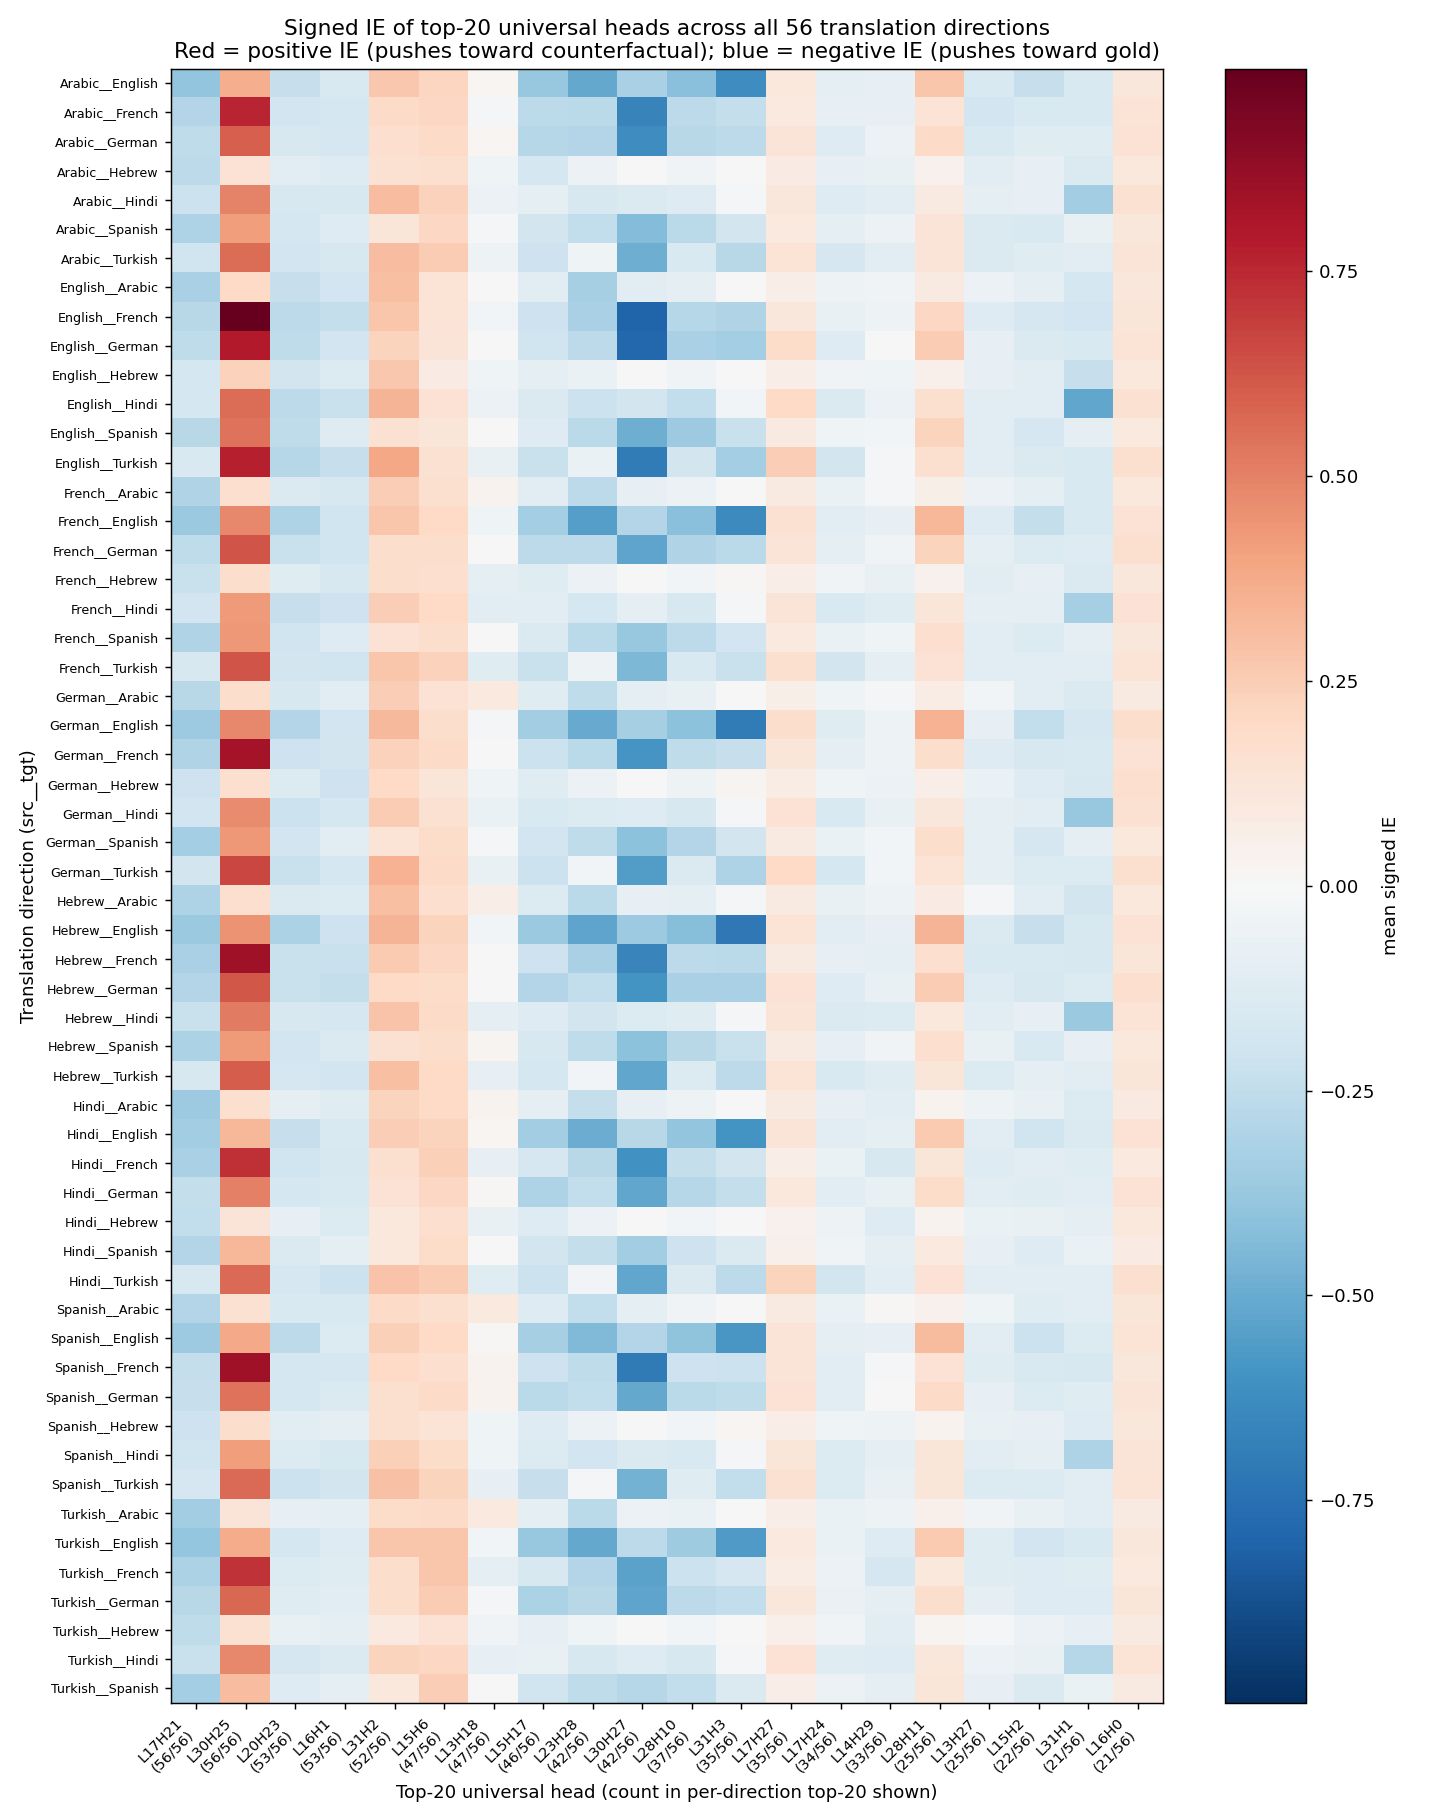
\includegraphics[width=\linewidth]{experiments/gcm_translation/img/meeting_direction_by_universal_head_signed.png}
\caption{Signed IE of the top-$20$ universal heads across all $56$
cross-language directions ($K{=}20$, from
\texttt{analyze.py --top\_k\_for\_universality 20}). Red cells indicate positive
IE (the head's original state pushes toward the counterfactual response); blue
cells indicate negative IE (pushes toward the gold response). The plot makes the
head-level caveat visible: high reuse counts do not imply translation-specificity
after the null controls (cf.\ Fig.~\ref{fig:gcm-decomp}). Produced by
\texttt{meeting\_plots.py}.}
\label{fig:gcm-signed-heads}
\end{figure}

\subsection{Signed GCM head groups predict monolingual grammatical effects}
\label{sec:gcm-ablate}

If translation reuses language-modeling machinery, the heads GCM implicates for
\emph{translation} should also matter for \emph{monolingual} grammaticality.

\paragraph{Method.} For each target language $L$ we aggregate GCM head effects
over the seven directions \emph{into} $L$ (excluding $L\!\to\!L$), taking the
per-pair mean of both $|\widehat{\mathrm{IE}}|$ and signed
$\widehat{\mathrm{IE}}$, and select the top-$20$ heads by aggregated mean
absolute IE. We then split this set by the sign of the aggregated signed IE into
a \textsc{pos} and a \textsc{neg} sub-population. We score each Multi-BLiMP
minimal pair by $\Delta = \log p(\text{correct final token}) -
\log p(\text{incorrect final token})$ at the prefix-final position, and report
$\Delta_{\text{change}} = \Delta_{\text{ablation}} - \Delta_{\text{baseline}}$
under mean-ablation of a head set (replacing the head's \texttt{o\_proj.input}
slice with its position-averaged language mean, applied via the equivalent
output delta). A negative $\Delta_{\text{change}}$ means ablation weakened the
grammaticality margin; positive means it strengthened it. Controls are
stratified same-layer random heads. We run six languages at $n{=}400$ and two
(heb, hin) at $n{=}200$.

\paragraph{Result: GCM sign predicts the monolingual ablation effect.} In all
eight languages, ablating the \textsc{neg}-signed sub-population
\emph{weakened} the grammaticality margin ($\Delta_{\text{change}}$ from $-0.12$
to $-1.02$), while ablating the \textsc{pos}-signed sub-population
\emph{strengthened} it ($+0.05$ to $+0.22$). A property measured purely in the
translation task---the sign of a head's GCM indirect effect---thus predicts the
direction of its causal effect on a monolingual grammaticality task. The
\textsc{neg}-signed heads (the majority, $\sim$65--80\% of the top-$20$) behave
like shared language-modeling machinery that translation borrows; the smaller
\textsc{pos}-signed population behaves like translation-specific routing, whose
removal does not carry monolingual grammaticality information. By contrast, the
mixed top-$5$ collective and the random controls are at the noise floor in
$7/8$ languages, because a set chosen by absolute IE alone mixes the two
opposing populations.

\begin{figure}[t]
\centering
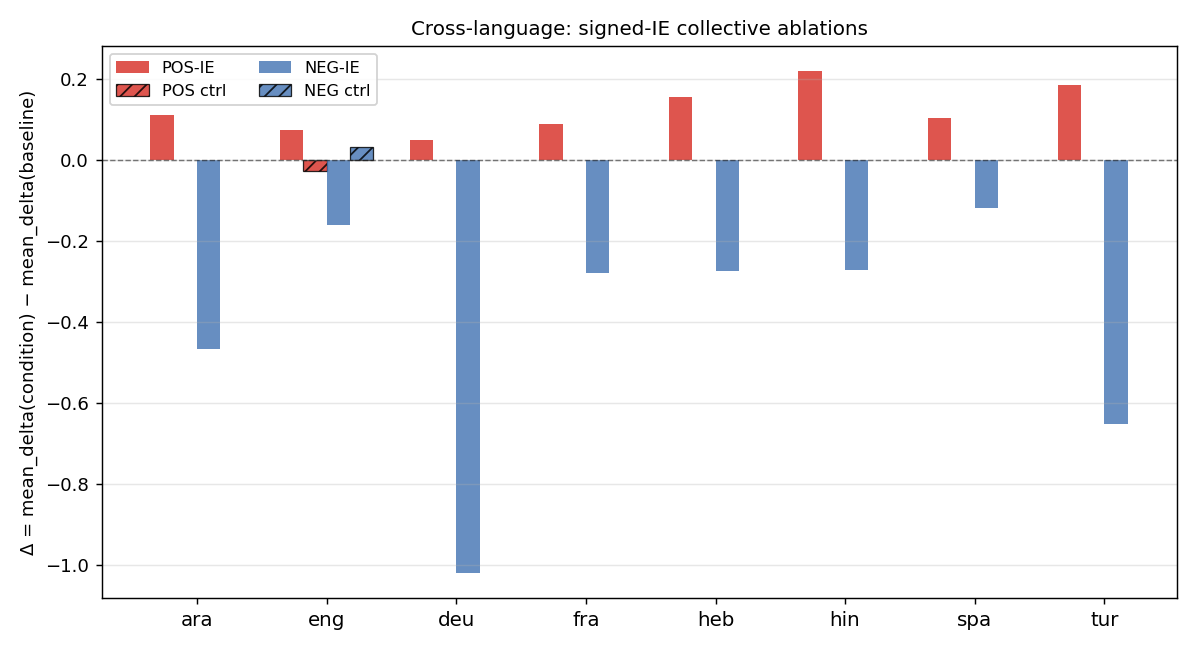
\includegraphics[width=\linewidth]{experiments/head_ablation_multiblimp/img/cross_lang_sign_split.png}
\caption{Per-language $\Delta_{\text{change}}$ on Multi-BLiMP from ablating the
\textsc{pos}-signed vs.\ \textsc{neg}-signed sub-population of the top-$20$ GCM
heads. Negative means ablation weakened the grammaticality preference. Produced
by \texttt{visualize.py} from \texttt{analysis\_summary.csv}.
\jb{Add the size-matched random controls (already coded in run.py; need a rerun
off the sm\_120 nodes) before this is submission-ready; see PAPER\_TODO A3. Full
per-condition table $\to$ appendix.}}
\label{fig:ablate-signsplit}
\end{figure}

\jb{Open caveats to fold into Limitations: (i) head-level translation-circuit
contributions in \S\ref{sec:gcm-id} are at the bf16 noise floor---the
feature-level evidence is the stronger claim; (ii) head selection here uses the
pre-control Phase-1 ranking; (iii) several $\Delta_{\text{change}}$ values are
within 2--3$\times$ of the noise floor; (iv) heb/hin at $n{=}200$; (v) the
size-matched sign-split controls are pending.}

% =====================================================================
\section{Monolingual Finetuning Is Competitive With Parallel Corpora}
\label{sec:finetune}
\jb{External (Jannik). Prose + figures to be supplied; states H3.}

\section{Discussion and Conclusions}
\jb{From v4.tex: the three results are convergent, not conclusive, evidence that
translation reuses language-modeling machinery through a multilingual semantic
hub. Emphasize that translation-selective mechanisms surely also exist; our aim
is to explain why monolingual pretraining helps translation at all.}

\section*{Limitations}
\jb{All interpretability results are Llama-3.1-8B with a single layer-16 SAE on a
base (non-instruction-tuned) model; Aya appears only in \S\ref{sec:linear}.
Plus the head-level / noise-floor / sample-size caveats noted above. The H2
input-output overlap result is also weak in the current saved outputs: across
the 25 cells with usable vectors, mean Jaccard@200 is only 0.095 using raw
scores and 0.122 using absolute-magnitude scores; several cells are missing or
malformed.}

\bibliographystyle{acl_natbib}
\bibliography{custom}
% Bib keys to add: sankaranarayanan2026gcm (arXiv:2602.16080),
% goyal2022flores, jumelet2025multiblimp.

\appendix
\section{Full head-ablation results}

\begin{figure}[h]
\centering
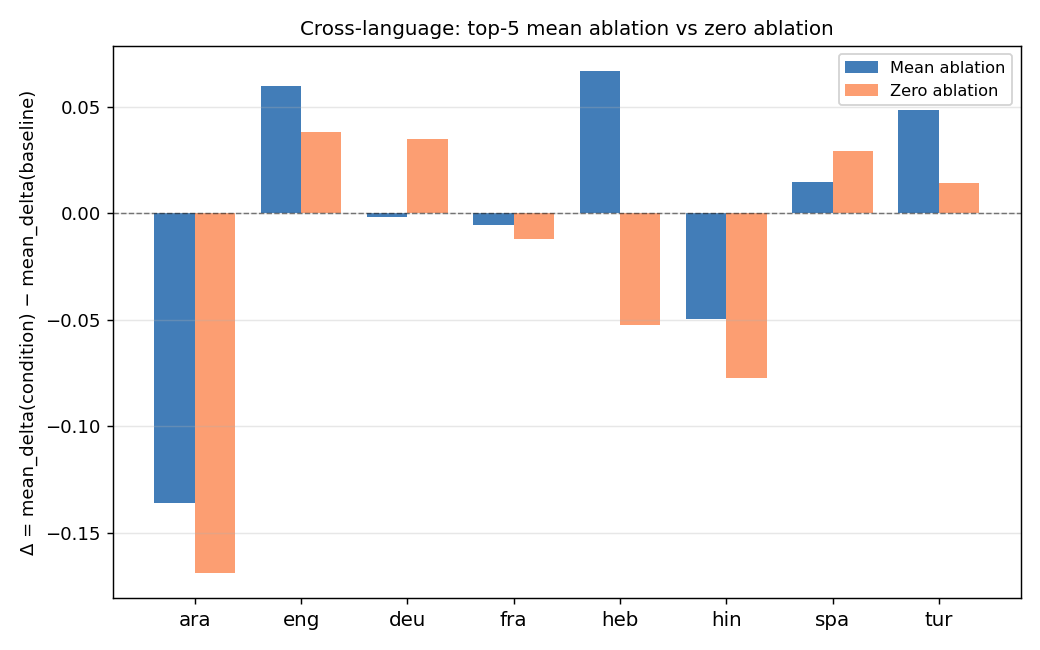
\includegraphics[width=\linewidth]{experiments/head_ablation_multiblimp/img/cross_lang_mean_vs_zero.png}
\caption{Appendix figure: mean-ablation versus zero-ablation for the top-$5$
GCM-head collective across target languages.}
\end{figure}

\begin{figure}[h]
\centering

\includegraphics[width=.49\linewidth]{experiments/gcm_translation/img/heads_heatmap/English__Spanish_heads_heatmap.png}

\includegraphics[width=.49\linewidth]{experiments/gcm_translation/img/heads_signed_heatmap/English__Spanish_heads_signed_heatmap.png}
\caption{Appendix method illustration for English$\to$Spanish GCM: mean
$|\widehat{\mathrm{IE}}|$ over heads (left) and signed mean IE (right).}
\end{figure}

\jb{Full per-condition table lives at
\texttt{outputs/head\_ablation\_multiblimp/analysis\_summary.csv}; convert to a
LaTeX table after the queued v2 matched-control rerun completes.}

\end{document}
